\chapter{Multi Qubit Gates}

When we move from operations on a single qubit to operations that take in multiple qubits as inputs we gain much more flexibility. One particular type of operation is of great interest to us, a controlled operation. Classical computation is full of conditionals of the form "If A then do B" and we would like to have something similar for quantum circuits as well. Let's start with the simplest of them all, Controlled NOT gates.

\section{The Controlled NOT Gate}

The controlled NOT gate takes in two qubits. One is termed as the control qubit and the other is termed as the target qubit. The control qubit is responsible for controlling the operation on the target qubit and operation that we seek to achieve is the NOT operation. In a circuit CNOT is represented in the following manner:


\begin{figure}[htp]
    \centering
    
\includegraphics[width=\textwidth]{cnot}
\end{figure}

The upper qubit is the control qubit and the lower one is the target. If the upper qubit is in $\ket{1}$ state then the NOT gate is applied on the lower qubit. Thus a state $\ket{10}$ on being sent to through this gate will turn into $\ket{11}$ while a state $\ket{01}$ will remain $\ket{01}$.

\section{Universality of CNOT}
This simple gate is extremely powerful as using just a CNOT gate and some single qubit gates we can implement any other multi qubit gate. In a sense the CNOT gate is a universal gate which we need in order to construct gates that perform unitary operations on multiple qubits.

As a simple example showing how this construction can be applied in practice let us see how a controlled-$U$ gate can be implemented using just single qubit gates and a CNOT gate. Single qubit gates on their own can be implemented using the universal single qubit gates and so we will assume that they can be implemented.

Recall from Exercise 5.3 that any single qubit gate can be written in the form $U = e^{i\alpha}AXBXC$ where $ABC = I$ with $A, B, C$ being three single qubit gates.
Consider the following construction. It is left as a trivial exercise to verify that the right hand circuit is indeed implementing the left hand controlled U operation.

\begin{figure}[htp]
    \centering
    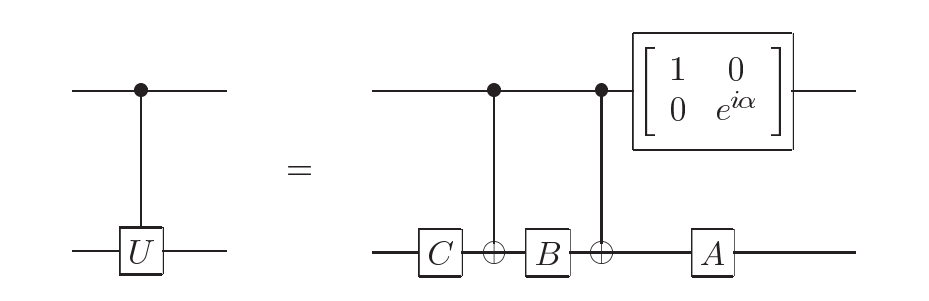
\includegraphics[width=\textwidth]{construct}
\end{figure}

We can also have gates that have more than a single qubit as their control qubit. A controlled $U$ gate with $n$ controls is represented as $C^n(U)$

\begin{exercise}
Prove that a $C^2(U)$ gate (for any single qubit unitary $U$) can be
constructed using at most eight one-qubit gates, and six CNOT gates
\end{exercise}

A lot can be said about multi qubit gates but essentially the main point is that it can be proven that any unitary operation on multiple qubits can be achieved upto arbitrary accuracy using hadamard, phase, CNOT, and $\pi/8$ gates. The proof is a bit involved and we skip it but the main idea is that any unitary operation on multiple qubits can be expressed as a product of unitary operators that operate on two or less qubits. Thus if we show that we can construct any unitary operator acting on two or less qubits we are done. It is then proven that single qubit gates with CNOT gates are sufficient to implement any arbitary gate operating on two qubits. Finally we have to show that any single qubit gate can be approximated using some fixed universal gates that we mentioned above. Although it is theoretically proven implementing everything that we have discussed in practice seems quite complicated and this is one of the main challenges that physicists and computer scientists have been working on in order to bring quantum computation to fruition.

We now move onto actually discussing and talking about some quantum algorithms. We will begin with some simple quantum algorithms and make our way towards Quantum Fourier Transform and Quantum Search based algorithms.
\clearpage